
%% bare_conf.tex
%% V1.3
%% 2007/01/11
%% by Michael Shell
%% See:
%% http://www.michaelshell.org/
%% for current contact information.
%%
%% This is a skeleton file demonstrating the use of IEEEtran.cls
%% (requires IEEEtran.cls version 1.7 or later) with an IEEE conference paper.
%%
%% Support sites:
%% http://www.michaelshell.org/tex/ieeetran/
%% http://www.ctan.org/tex-archive/macros/latex/contrib/IEEEtran/
%% and
%% http://www.ieee.org/

%%*************************************************************************
%% Legal Notice:
%% This code is offered as-is without any warranty either expressed or
%% implied; without even the implied warranty of MERCHANTABILITY or
%% FITNESS FOR A PARTICULAR PURPOSE! 
%% User assumes all risk.
%% In no event shall IEEE or any contributor to this code be liable for
%% any damages or losses, including, but not limited to, incidental,
%% consequential, or any other damages, resulting from the use or misuse
%% of any information contained here.
%%
%% All comments are the opinions of their respective authors and are not
%% necessarily endorsed by the IEEE.
%%
%% This work is distributed under the LaTeX Project Public License (LPPL)
%% ( http://www.latex-project.org/ ) version 1.3, and may be freely used,
%% distributed and modified. A copy of the LPPL, version 1.3, is included
%% in the base LaTeX documentation of all distributions of LaTeX released
%% 2003/12/01 or later.
%% Retain all contribution notices and credits.
%% ** Modified files should be clearly indicated as such, including  **
%% ** renaming them and changing author support contact information. **
%%
%% File list of work: IEEEtran.cls, IEEEtran_HOWTO.pdf, bare_adv.tex,
%%                    bare_conf.tex, bare_jrnl.tex, bare_jrnl_compsoc.tex
%%*************************************************************************

% *** Authors should verify (and, if needed, correct) their LaTeX system  ***
% *** with the testflow diagnostic prior to trusting their LaTeX platform ***
% *** with production work. IEEE's font choices can trigger bugs that do  ***
% *** not appear when using other class files.                            ***
% The testflow support page is at:
% http://www.michaelshell.org/tex/testflow/



% Note that the a4paper option is mainly intended so that authors in
% countries using A4 can easily print to A4 and see how their papers will
% look in print - the typesetting of the document will not typically be
% affected with changes in paper size (but the bottom and side margins will).
% Use the testflow package mentioned above to verify correct handling of
% both paper sizes by the user's LaTeX system.
%
% Also note that the "draftcls" or "draftclsnofoot", not "draft", option
% should be used if it is desired that the figures are to be displayed in
% draft mode.
%
\documentclass[conference]{IEEEtran}
% Add the compsoc option for Computer Society conferences.
%
% If IEEEtran.cls has not been installed into the LaTeX system files,
% manually specify the path to it like:
% \documentclass[conference]{../sty/IEEEtran}


\usepackage{cite}



% Some very useful LaTeX packages include:
% (uncomment the ones you want to load)


% *** MISC UTILITY PACKAGES ***
%
%\usepackage{ifpdf}
% Heiko Oberdiek's ifpdf.sty is very useful if you need conditional
% compilation based on whether the output is pdf or dvi.
% usage:
% \ifpdf
%   % pdf code
% \else
%   % dvi code
% \fi
% The latest version of ifpdf.sty can be obtained from:
% http://www.ctan.org/tex-archive/macros/latex/contrib/oberdiek/
% Also, note that IEEEtran.cls V1.7 and later provides a builtin
% \ifCLASSINFOpdf conditional that works the same way.
% When switching from latex to pdflatex and vice-versa, the compiler may
% have to be run twice to clear warning/error messages.






% *** CITATION PACKAGES ***
%
%\usepackage{cite}
% cite.sty was written by Donald Arseneau
% V1.6 and later of IEEEtran pre-defines the format of the cite.sty package
% \cite{} output to follow that of IEEE. Loading the cite package will
% result in citation numbers being automatically sorted and properly
% "compressed/ranged". e.g., [1], [9], [2], [7], [5], [6] without using
% cite.sty will become [1], [2], [5]--[7], [9] using cite.sty. cite.sty's
% \cite will automatically add leading space, if needed. Use cite.sty's
% noadjust option (cite.sty V3.8 and later) if you want to turn this off.
% cite.sty is already installed on most LaTeX systems. Be sure and use
% version 4.0 (2003-05-27) and later if using hyperref.sty. cite.sty does
% not currently provide for hyperlinked citations.
% The latest version can be obtained at:
% http://www.ctan.org/tex-archive/macros/latex/contrib/cite/
% The documentation is contained in the cite.sty file itself.






% *** GRAPHICS RELATED PACKAGES ***
%
\ifCLASSINFOpdf
  \usepackage[pdftex]{graphicx}
  \usepackage{caption}
  \usepackage{subcaption}
  %\usepackage{filecontents}
  % declare the path(s) where your graphic files are
  % \graphicspath{{../pdf/}{../jpeg/}}
  % and their extensions so you won't have to specify these with
  % every instance of \includegraphics
  % \DeclareGraphicsExtensions{.pdf,.jpeg,.png}
\else
  % or other class option (dvipsone, dvipdf, if not using dvips). graphicx
  % will default to the driver specified in the system graphics.cfg if no
  % driver is specified.
  % \usepackage[dvips]{graphicx}
  % declare the path(s) where your graphic files are
  % \graphicspath{{../eps/}}
  % and their extensions so you won't have to specify these with
  % every instance of \includegraphics
  % \DeclareGraphicsExtensions{.eps}
\fi
% graphicx was written by David Carlisle and Sebastian Rahtz. It is
% required if you want graphics, photos, etc. graphicx.sty is already
% installed on most LaTeX systems. The latest version and documentation can
% be obtained at: 
% http://www.ctan.org/tex-archive/macros/latex/required/graphics/
% Another good source of documentation is "Using Imported Graphics in
% LaTeX2e" by Keith Reckdahl which can be found as epslatex.ps or
% epslatex.pdf at: http://www.ctan.org/tex-archive/info/
%
% latex, and pdflatex in dvi mode, support graphics in encapsulated
% postscript (.eps) format. pdflatex in pdf mode supports graphics
% in .pdf, .jpeg, .png and .mps (metapost) formats. Users should ensure
% that all non-photo figures use a vector format (.eps, .pdf, .mps) and
% not a bitmapped formats (.jpeg, .png). IEEE frowns on bitmapped formats
% which can result in "jaggedy"/blurry rendering of lines and letters as
% well as large increases in file sizes.
%
% You can find documentation about the pdfTeX application at:
% http://www.tug.org/applications/pdftex





% *** MATH PACKAGES ***
%
\usepackage[cmex10]{amsmath}
\usepackage{amsthm}
% A popular package from the American Mathematical Society that provides
% many useful and powerful commands for dealing with mathematics. If using
% it, be sure to load this package with the cmex10 option to ensure that
% only type 1 fonts will utilized at all point sizes. Without this option,
% it is possible that some math symbols, particularly those within
% footnotes, will be rendered in bitmap form which will result in a
% document that can not be IEEE Xplore compliant!
%
% Also, note that the amsmath package sets \interdisplaylinepenalty to 10000
% thus preventing page breaks from occurring within multiline equations. Use:
%\interdisplaylinepenalty=2500
% after loading amsmath to restore such page breaks as IEEEtran.cls normally
% does. amsmath.sty is already installed on most LaTeX systems. The latest
% version and documentation can be obtained at:
% http://www.ctan.org/tex-archive/macros/latex/required/amslatex/math/



% *** TIKZ PACKAGES
%
\usepackage[svgnames]{xcolor}
\usepackage{tikz}
\tikzstyle{none}=[inner sep=0pt]
\tikzstyle{arrow}=[-latex,draw=Black,line width=0.75]
\tikzstyle{simple}=[-,draw=Black]





% *** SPECIALIZED LIST PACKAGES ***
%
%\usepackage{algorithmic}
% algorithmic.sty was written by Peter Williams and Rogerio Brito.
% This package provides an algorithmic environment fo describing algorithms.
% You can use the algorithmic environment in-text or within a figure
% environment to provide for a floating algorithm. Do NOT use the algorithm
% floating environment provided by algorithm.sty (by the same authors) or
% algorithm2e.sty (by Christophe Fiorio) as IEEE does not use dedicated
% algorithm float types and packages that provide these will not provide
% correct IEEE style captions. The latest version and documentation of
% algorithmic.sty can be obtained at:
% http://www.ctan.org/tex-archive/macros/latex/contrib/algorithms/
% There is also a support site at:
% http://algorithms.berlios.de/index.html
% Also of interest may be the (relatively newer and more customizable)
% algorithmicx.sty package by Szasz Janos:
% http://www.ctan.org/tex-archive/macros/latex/contrib/algorithmicx/




% *** ALIGNMENT PACKAGES ***
%
%\usepackage{array}
% Frank Mittelbach's and David Carlisle's array.sty patches and improves
% the standard LaTeX2e array and tabular environments to provide better
% appearance and additional user controls. As the default LaTeX2e table
% generation code is lacking to the point of almost being broken with
% respect to the quality of the end results, all users are strongly
% advised to use an enhanced (at the very least that provided by array.sty)
% set of table tools. array.sty is already installed on most systems. The
% latest version and documentation can be obtained at:
% http://www.ctan.org/tex-archive/macros/latex/required/tools/


%\usepackage{mdwmath}
%\usepackage{mdwtab}
% Also highly recommended is Mark Wooding's extremely powerful MDW tools,
% especially mdwmath.sty and mdwtab.sty which are used to format equations
% and tables, respectively. The MDWtools set is already installed on most
% LaTeX systems. The lastest version and documentation is available at:
% http://www.ctan.org/tex-archive/macros/latex/contrib/mdwtools/


% IEEEtran contains the IEEEeqnarray family of commands that can be used to
% generate multiline equations as well as matrices, tables, etc., of high
% quality.


%\usepackage{eqparbox}
% Also of notable interest is Scott Pakin's eqparbox package for creating
% (automatically sized) equal width boxes - aka "natural width parboxes".
% Available at:
% http://www.ctan.org/tex-archive/macros/latex/contrib/eqparbox/





% *** SUBFIGURE PACKAGES ***
%\usepackage[tight,footnotesize]{subfigure}
% subfigure.sty was written by Steven Douglas Cochran. This package makes it
% easy to put subfigures in your figures. e.g., "Figure 1a and 1b". For IEEE
% work, it is a good idea to load it with the tight package option to reduce
% the amount of white space around the subfigures. subfigure.sty is already
% installed on most LaTeX systems. The latest version and documentation can
% be obtained at:
% http://www.ctan.org/tex-archive/obsolete/macros/latex/contrib/subfigure/
% subfigure.sty has been superceeded by subfig.sty.



%\usepackage[caption=false]{caption}
%\usepackage[font=footnotesize]{subfig}
% subfig.sty, also written by Steven Douglas Cochran, is the modern
% replacement for subfigure.sty. However, subfig.sty requires and
% automatically loads Axel Sommerfeldt's caption.sty which will override
% IEEEtran.cls handling of captions and this will result in nonIEEE style
% figure/table captions. To prevent this problem, be sure and preload
% caption.sty with its "caption=false" package option. This is will preserve
% IEEEtran.cls handing of captions. Version 1.3 (2005/06/28) and later 
% (recommended due to many improvements over 1.2) of subfig.sty supports
% the caption=false option directly:
%\usepackage[caption=false,font=footnotesize]{subfig}
%
% The latest version and documentation can be obtained at:
% http://www.ctan.org/tex-archive/macros/latex/contrib/subfig/
% The latest version and documentation of caption.sty can be obtained at:
% http://www.ctan.org/tex-archive/macros/latex/contrib/caption/




% *** FLOAT PACKAGES ***
%
%\usepackage{fixltx2e}
% fixltx2e, the successor to the earlier fix2col.sty, was written by
% Frank Mittelbach and David Carlisle. This package corrects a few problems
% in the LaTeX2e kernel, the most notable of which is that in current
% LaTeX2e releases, the ordering of single and double column floats is not
% guaranteed to be preserved. Thus, an unpatched LaTeX2e can allow a
% single column figure to be placed prior to an earlier double column
% figure. The latest version and documentation can be found at:
% http://www.ctan.org/tex-archive/macros/latex/base/



%\usepackage{stfloats}
% stfloats.sty was written by Sigitas Tolusis. This package gives LaTeX2e
% the ability to do double column floats at the bottom of the page as well
% as the top. (e.g., "\begin{figure*}[!b]" is not normally possible in
% LaTeX2e). It also provides a command:
%\fnbelowfloat
% to enable the placement of footnotes below bottom floats (the standard
% LaTeX2e kernel puts them above bottom floats). This is an invasive package
% which rewrites many portions of the LaTeX2e float routines. It may not work
% with other packages that modify the LaTeX2e float routines. The latest
% version and documentation can be obtained at:
% http://www.ctan.org/tex-archive/macros/latex/contrib/sttools/
% Documentation is contained in the stfloats.sty comments as well as in the
% presfull.pdf file. Do not use the stfloats baselinefloat ability as IEEE
% does not allow \baselineskip to stretch. Authors submitting work to the
% IEEE should note that IEEE rarely uses double column equations and
% that authors should try to avoid such use. Do not be tempted to use the
% cuted.sty or midfloat.sty packages (also by Sigitas Tolusis) as IEEE does
% not format its papers in such ways.





% *** PDF, URL AND HYPERLINK PACKAGES ***
%
%\usepackage{url}
% url.sty was written by Donald Arseneau. It provides better support for
% handling and breaking URLs. url.sty is already installed on most LaTeX
% systems. The latest version can be obtained at:
% http://www.ctan.org/tex-archive/macros/latex/contrib/misc/
% Read the url.sty source comments for usage information. Basically,
% \url{my_url_here}.





% *** Do not adjust lengths that control margins, column widths, etc. ***
% *** Do not use packages that alter fonts (such as pslatex).         ***
% There should be no need to do such things with IEEEtran.cls V1.6 and later.
% (Unless specifically asked to do so by the journal or conference you plan
% to submit to, of course. )

% Thms
\newtheorem{thm}{Theorem}[section]
\newtheorem{theorem}[thm]{Theorem}
\newtheorem{corollary}[thm]{Corollary}
\newtheorem{proposition}[thm]{Proposition}

% Defs
\theoremstyle{definition}
\newtheorem{definition}[thm]{Definition}
\newtheorem{example}[thm]{Example}
\newtheorem{assumption}[thm]{Assumption}

% Proofs
%\newtheorem{Pf}{Proof$\!\!$}         \renewcommand{\thePf}{}
%\newenvironment{pf}{\begin{Pf}}{\qed\end{Pf}}

%\newtheorem{ques}[thm]{Question}





% correct bad hyphenation here
\hyphenation{op-tical net-works semi-conduc-tor}


\begin{document}
%
% paper title
% can use linebreaks \\ within to get better formatting as desired
\title{Topic 1: A Better UDP}


% author names and affiliations
% use a multiple column layout for up to three different
% affiliations
\author{\IEEEauthorblockN{Carson Clanton}
\IEEEauthorblockA{\small Department of Computer\\Science and Engineering\\
The University of Texas\\at Arlington\\
Arlington, Texas 76019\\
clanton@uta.edu}
\and
\IEEEauthorblockN{Kevin Hayes}
\IEEEauthorblockA{\small Department of Computer\\Science and Engineering\\
The University of Texas\\at Arlington\\
Arlington, Texas 76019\\
kevin.hayes@mavs.uta.edu}
\and
\IEEEauthorblockN{William Hunter}
\IEEEauthorblockA{\small Department of Computer\\Science and Engineering\\
The University of Texas\\at Arlington\\
Arlington, Texas 76019\\
whunter@mavs.uta.edu}
\and
\IEEEauthorblockN{Richard Meth}
\IEEEauthorblockA{\small Department of Computer\\Science and Engineering\\
The University of Texas\\at Arlington\\
Arlington, Texas 76019\\
richard.meth@mavs.uta.edu}
\and
\IEEEauthorblockN{Ryan Nordeen}
\IEEEauthorblockA{\small Department of Computer\\Science and Engineering\\
The University of Texas\\at Arlington\\
Arlington, Texas 76019\\
ryan.nordeen@mavs.uta.edu}
}

% conference papers do not typically use \thanks and this command
% is locked out in conference mode. If really needed, such as for
% the acknowledgment of grants, issue a \IEEEoverridecommandlockouts
% after \documentclass

% for over three affiliations, or if they all won't fit within the width
% of the page, use this alternative format:
% 
%\author{\IEEEauthorblockN{Michael Shell\IEEEauthorrefmark{1},
%Homer Simpson\IEEEauthorrefmark{2},
%James Kirk\IEEEauthorrefmark{3}, 
%Montgomery Scott\IEEEauthorrefmark{3} and
%Eldon Tyrell\IEEEauthorrefmark{4}}
%\IEEEauthorblockA{\IEEEauthorrefmark{1}School of Electrical and Computer Engineering\\
%Georgia Institute of Technology,
%Atlanta, Georgia 30332--0250\\ Email: see http://www.michaelshell.org/contact.html}
%\IEEEauthorblockA{\IEEEauthorrefmark{2}Twentieth Century Fox, Springfield, USA\\
%Email: homer@thesimpsons.com}
%\IEEEauthorblockA{\IEEEauthorrefmark{3}Starfleet Academy, San Francisco, California 96678-2391\\
%Telephone: (800) 555--1212, Fax: (888) 555--1212}
%\IEEEauthorblockA{\IEEEauthorrefmark{4}Tyrell Inc., 123 Replicant Street, Los Angeles, California 90210--4321}}




% use for special paper notices
%\IEEEspecialpapernotice{(Invited Paper)}




% make the title area
\maketitle


\begin{abstract}
%\boldmath
This article describes an approach to improving the reliability of UDP.
Our approach uses sequence numbers for datagrams to force in-order delivery
to the Network Application layer and Error-Correcting Codes to help reproduce
lost datagrams without requesting retransmission of these missing datagrams.  The
level of data reconstruction will be largely dependent on the Error-Correcting
Code chosen and the selection of its associated redundancy parameters.
\end{abstract}
% IEEEtran.cls defaults to using nonbold math in the Abstract.
% This preserves the distinction between vectors and scalars. However,
% if the conference you are submitting to favors bold math in the abstract,
% then you can use LaTeX's standard command \boldmath at the very start
% of the abstract to achieve this. Many IEEE journals/conferences frown on
% math in the abstract anyway.

% no keywords




% For peer review papers, you can put extra information on the cover
% page as needed:
% \ifCLASSOPTIONpeerreview
% \begin{center} \bfseries EDICS Category: 3-BBND \end{center}
% \fi
%
% For peerreview papers, this IEEEtran command inserts a page break and
% creates the second title. It will be ignored for other modes.
\IEEEpeerreviewmaketitle



\section{Introduction}
% no \IEEEPARstart
When a software engineer begins designing a
network application, he or she has to make a decision between
two transport layer options, TCP or UDP \cite{kurose2012computer}.
There are advantages and disadvantages to both.  With UDP comes
nimbleness and low overhead, along with dropped and possibly
out-of-sequence datagrams.  With TCP comes reliable stream-based
communication at the expense of throughput.  There isn't much
middle ground between the two.  The approach discussed in this
paper attempts to change that.
% You must have at least 2 lines in the paragraph with the drop letter
% (should never be an issue)

We don't attempt or intend to redesign either protocol.  Instead,
we seek to enhance the reliability of UDP, so that it is a little
more like TCP, while remaining connectionless.  To do this, we
will require two added features to be built ``on top'' of UDP:
Sequence Numbers and Error-Correcting Codes.

The introduction of sequence numbers should be somewhat obvious;
on the receiving end of the UDP pathway there should be someway
to put datagrams back in order.  The subtlety, however, of requiring
sequence numbers is that in order for our error-correcting codes
approach to work, for the code we experimented with, at least 75\%
of the datagram payload data must be available and properly
sequenced.  So, the inclusion of sequence numbers is twofold.

The second feature to be added, Error-Correcting Codes or ECC, is a
little more complicated and requires more of an introduction,
if for no other reason than to get acclimated to the terminology
in the literature.

Given the no-guaranty and low-reliability characteristics of
the networking layer and the little added value of UDP,
a virtual communication link through a UDP socket represents
an unreliable, and potentially noisy, channel, making it
a good candidate for a ECC solution.


\subsection{Error-Correcting Codes}
Below in Figure \ref{comm_link} is a block diagram of the general
communication link for sending messages \cite{clanton2005maa}.
Here the message is first sent by the \emph{source} to the
\emph{encoder} where the message is assigned a \emph{codeword},
i.e. a string of characters from some chosen alphabet.  The
encoded message is sent through a \emph{channel}, which is
certain to have some level of noise that may possibly alter
the codeword.  This possibly-altered codeword is then received
by the \emph{decoder} where it is matched with its most likely
candidate codeword which is in turn translated into a message
resembling the original message and passed on to the \emph{receiver}.
The degree of resemblance to the original message depends
on how appropriate the code is in relation to the channel.\\





%%%%************************************************************************%%%%
%%%%                                                                        %%%%
%%%%    COMMUNICATION LINK DIAGRAM - BEGIN                                  %%%%
%%%%                                                                        %%%%
%%%%                                                                        %%%%
                                                                            %%%%
\begin{figure}[!t]                                                          %%%%
\centering                                                                  %%%%
\resizebox{0.45\textwidth}{!}{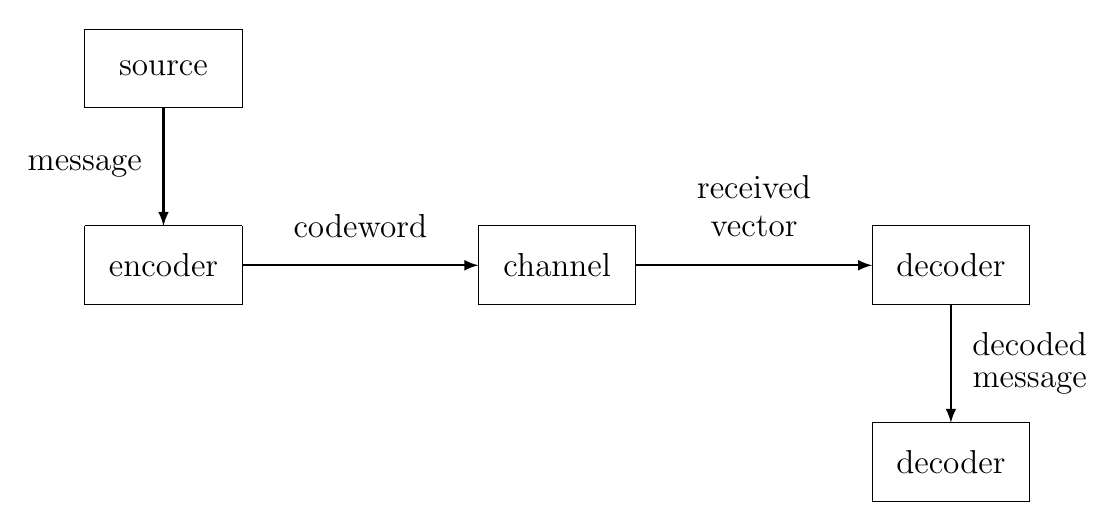
\begin{tikzpicture}
 \node [style=none] (0) at (-3, 1) {};                                 
 \node [style=none] (1) at (-5, 1) {};                                 
 \node [style=none] (2) at (-3, -0) {};                                
 \node [style=none] (3) at (-5, -0) {};                                
 \node [style=none] (4) at (-4, 0.5)     {\large source};         
 \node [style=none] (5) at (-3, 0.5) {};                               
 \node [style=none] (6) at (-5, 0.5) {};                               
 \node [style=none] (7) at (-4, 1) {};                                 
 \node [style=none] (8) at (-4, -0) {};                                
 \node [style=none] (9) at (-5, -2.5) {};                              
 \node [style=none] (10) at (-3, -1.5) {};                             
 \node [style=none] (11) at (-5, -2) {};                               
 \node [style=none] (12) at (-4, -2.5) {};                             
 \node [style=none] (13) at (-5, -1.5) {};                             
 \node [style=none] (14) at (-4, -2)     {\large encoder};        
 \node [style=none] (15) at (-4, -1.5) {};                             
 \node [style=none] (16) at (-3, -2.5) {};                             
 \node [style=none] (17) at (-3, -2) {};                               
 \node [style=none] (18) at (1, -2)      {\large channel};        
 \node [style=none] (19) at (2, -2) {};                                
 \node [style=none] (20) at (2, -2.5) {};                              
 \node [style=none] (21) at (0, -2) {};                                
 \node [style=none] (22) at (0, -2.5) {};                              
 \node [style=none] (23) at (1, -2.5) {};                              
 \node [style=none] (24) at (0, -1.5) {};                              
 \node [style=none] (25) at (2, -1.5) {};                              
 \node [style=none] (26) at (1, -1.5) {};                              
 \node [style=none] (27) at (6, -2)      {\large decoder};        
 \node [style=none] (28) at (7, -1.5) {};                              
 \node [style=none] (29) at (6, -1.5) {};                              
 \node [style=none] (30) at (7, -2) {};                                
 \node [style=none] (31) at (7, -2.5) {};                              
 \node [style=none] (32) at (5, -2) {};                                
 \node [style=none] (33) at (5, -2.5) {};                              
 \node [style=none] (34) at (5, -1.5) {};                              
 \node [style=none] (35) at (6, -2.5) {};                              
 \node [style=none] (36) at (5, -5) {};                                
 \node [style=none] (37) at (6, -4.5)    {\large decoder};        
 \node [style=none] (38) at (7, -5) {};                                
 \node [style=none] (39) at (7, -4.5) {};                              
 \node [style=none] (40) at (7, -4) {};                                
 \node [style=none] (41) at (5, -4.5) {};                              
 \node [style=none] (42) at (6, -4) {};                                
 \node [style=none] (43) at (5, -4) {};                                
 \node [style=none] (44) at (6, -5) {};                                
 \node [style=none] (45) at (-5, -0.75)  {\large message};        
 \node [style=none] (46) at (-1.5, -1.5) {\large codeword};       
 \node [style=none] (47) at (3.5, -1)    {\large received};       
 \node [style=none] (48) at (3.5, -1.5)  {\large vector};         
 \node [style=none] (49) at (7, -3)      {\large decoded};        
 \node [style=none] (50) at (7, -3.5)    {\large message};        
 \draw (1.center) to (3.center);                                       
 \draw (1.center) to (0.center);                                       
 \draw (3.center) to (2.center);                                       
 \draw (2.center) to (0.center);                                       
 \draw (13.center) to (9.center);                                      
 \draw (13.center) to (10.center);                                     
 \draw (9.center) to (16.center);                                      
 \draw (16.center) to (10.center);                                     
 \draw [style=arrow] (8.center) to (15.center);                        
 \draw (24.center) to (22.center);                                     
 \draw (24.center) to (25.center);                                     
 \draw (22.center) to (20.center);                                     
 \draw (20.center) to (25.center);                                     
 \draw [style=arrow] (17.center) to (21.center);                       
 \draw (34.center) to (33.center);                                     
 \draw (34.center) to (28.center);                                     
 \draw (33.center) to (31.center);                                     
 \draw (31.center) to (28.center);                                     
 \draw [style=arrow] (19.center) to (32.center);                       
 \draw (43.center) to (36.center);                                     
 \draw (43.center) to (40.center);                                     
 \draw (36.center) to (38.center);                                     
 \draw (38.center) to (40.center);                                     
 \draw [style=arrow] (35.center) to (42.center);                       
\end{tikzpicture}                                                      
}
\caption{Block diagram of a general communication link}                     %%%%
\label{comm_link}                                                           %%%%
\end{figure}                                                                %%%%
%%%%                                                                        %%%%
%%%%                                                                        %%%%
%%%%    COMMUNICATION LINK DIAGRAM  - END                                   %%%%
%%%%                                                                        %%%%
%%%%************************************************************************%%%%





\begin{example}
\label{YES_or_NO}
Suppose we are using an alphabet containing only two symbols,
say 0 and 1 and we wish to send a message to a friend of either
``YES'' or ``NO''.  We first might consider encoding 1 for
``YES'' and 0 for ``NO''; however, if the codeword 0 is sent
and then altered by the channel to be received as 1, the
decoder will incorrectly pass the message ``YES'' to the receiver.
One way of improving the situation is to add redundancy by
repeating the symbol.  For instance, we might encode ``YES''
as the codeword 11 and ``NO'' as 00.  Now if ``NO'' is sent,
two errors would have to occur before the decoder returns
an incorrect message.  If one error occurs then the received
vector will either be 10 or 01, neither of which is a codeword.
At this point, the receiver might request a retransmission.
This is an example of a code in which one error may be detected.
To strengthen the code to be error-correcting we might increase
the redundancy by repeating the message five times.  Thus we
encode our message ``NO'' as 00000.  Perhaps the channels
interferes to cause the decoder to receive the vector 00110.
Using the method of nearest neighbor decoding the decoder
assesses the message and decides that of the two possible
codewords (i.e. 00000 and 11111) 00000 is more likely the
one originally sent and hence is correctly decoded as ``NO''.
\end{example}




%\begin{assumption}
%Implicit in our example are two assumptions.  First, we are
%assuming that each symbol is equally likely to occur.  Second,
%the probability of an error is less than $1/2$. These are
%important assumptions to be aware as they will serve as
%guiding principles in the remainder of this paper.
%\end{assumption}

\begin{definition}
Let $\mathbf{F}$ be a finite set, or {\bf alphabet}, of $q$
elements.  A $q$-{\bf ary code} $\mathbf{C}$ is a set of
finite sequences of symbols of $\mathbf{F}$, called {\bf codewords}
and written $x_1x_2\cdots x_n$, or $(x_1,x_2,\ldots,x_n)$,
where $x_i\in \mathbf{F}$ for $i = 1,\ldots,n$. If all the
sequences have the same length $n$, then $\mathbf{C}$ is a
{\bf block code} of {\bf block length} $n$.
\end{definition}

Given an alphabet $\mathbf{F}$, it is consistent with
terminology for vector spaces when $\mathbf{F}$ is a
field to denote the set of all sequences of length $n$
of elements of $\mathbf{F}$ by $\mathbf{F}^n$ and to
call these sequences vectors.  The member of $\mathbf{F}$
at the $i$th position of a vector is known as the coordinate
at $i$.



\begin{definition}
Let $v=(v_1,v_2,\ldots,v_n)$ and $w=(w_1,w_2,\ldots,w_n)$ be
two vectors in $\mathbf{F}^n$.  The {\bf Hamming distance},
$d(v,w)$, between $v$ and $w$ is the number of coordinate
places in which they differ:
$$
d(v,w)=\{i|v_i\neq w_i \}
$$

We will usually refer to the Hamming distance as simply the
{\bf distance} between two vectors.
\end{definition}

{\bf Nearest-neighbor decoding} is a method in which the
received vector is translated as the codeword of smallest
distance, whenever it is uniquely determined.  This method
maximizes the likelihood of correcting errors provide the
two assumptions mentioned above hold (i.e. probability of
an error $<1/2$ and each symbol is equally likely to be
transmitted).

\begin{definition}
The {\bf minimum distance} $d(\mathbf{C})$ of a code
$\mathbf{C}$ is the smallest of the distances between
distinct codewords; i.e.
$$
d(\mathbf{C}) = \min\{d(v,w)|v,w\in\mathbf{C},v\neq w\}
$$
\end{definition}


\begin{example}
The error-correcting code in Example \ref{YES_or_NO} is
a binary code of block length 5. The distance between
the codeword 00000 and the received vector 00110 is 2.
The distance between the same received vector and the
codeword 11111 is 3.  Thus, 00000 is the nearest neighboring
codeword.  The minimum distance of this code is 5.
\end{example}

\begin{definition}
A code $\mathbf{C}$ over $\mathbf{F}$ of length $n$ is
{\bf linear} if $\mathbf{C}$ is a subspace of the vector
space $V=\mathbf{F}^n$.  If $\dim(\mathbf{C})=k$ and
$d(\mathbf{C})=d$, then we write $[n,k,d]$ for the $q$-ary
code $\mathbf{C}$; if the minimum distance is not specified
we simply write $[n,k]$. The {\bf information rate} is $k/n$
and the {\bf redundancy} is $n-k$.  
\end{definition}

Since $\mathbf{C}$ is a subspace, it follows that the
{\bf all-zero} vector must be a codeword in $\mathbf{C}$
also the sum of any two codewords must also be a codeword
in $\mathbf{C}$.  We will also see after the next
definition that the distance $d$ is also easy to
calculate for linear codes.

\begin{definition}
Let $V=\mathbf{F}^n$.  For any vector $v=(v_1,v_2,\ldots,v_n)\in V$
set
$$
S=\left\{i|v_i\neq 0\right\}
$$
Then $S$ is called the support of $v$ and the weight of $v$ is
$\left|S\right|$.  The {\bf minimum weight} of a code is the
minimum of the weights of the nonzero codewords.
\end{definition}


\begin{example}\label{hamming}
Listed below are all 16 codewords in the linear $[7,4,3]$
binary code.  They are listed in order of increasing weight.\\

\begin{center}
 \begin{tabular}{cccc}
  0000000 & 0111000 & 1000111 & 0101101\\
  1100100 & 0001110 & 1101010 & 0110110\\
  1010010 & 0010101 & 1110001 & 0011011\\
  1001001 & 0100011 & 1011100 & 1111111\\
 \end{tabular}
\end{center}

Notice that the minimum weight is 3.  By Theorem 1.1 it
follows that $d(\mathbf{C}) = 3$.  It can be shown
that these 16 codewords form a subspace of $\mathbf{F}^7$
with basis $\{(1,0,0,0,1,1,1)$, $(0,1,0,0,0,1,1)$, 
$(0,0,1,0,1,0,1)$, $(0,0,0,1,1,1,0)\}$. Thus 
$\dim(\mathbf{C})=4$ as conveyed in the notation and the
redundancy is 3 since $n-k=7-4 = 3$.
\end{example}



\begin{theorem}
Let $\mathbf{C}$ be a code of minimum distance $d$.  If
$d\geq2t+1$, then $\mathbf{C}$ can be used to correct up
to $t$ errors.
\end{theorem}

\vspace{6pt}

\section{Design}
A Better UDP is ``wedged in'' as another IP stack
layer sitting between the transport layer and the application
layer, see Figure \ref{ip_stack}.  We did not modify any
kernel source and A Better UDP is not a standard yet, so
to use it an application developer or software engineer
will have to include this functionality as a library.
Instead of using a socket library to interface
with the transport layer, the engineer will link with
A Better UDP library to interface with the protocol stack
below the application layer. Henceforth we will refer
to A Better UDP as BUDP.



%%%%************************************************************************%%%%
%%%%                                                                        %%%%
%%%%    IP STACK DIAGRAM - BEGIN                                            %%%%
%%%%                                                                        %%%%
%%%%                                                                        %%%%
\begin{figure}[h!]                                                          %%%%
\centering                                                                  %%%%
\resizebox{0.150\textwidth}{!}{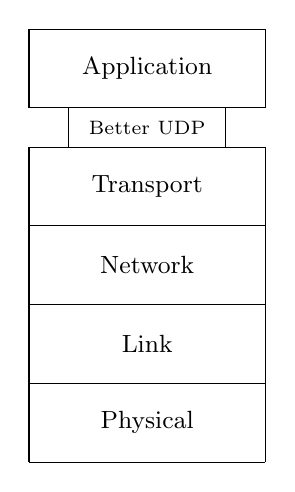
\begin{tikzpicture}
  \node [style=none] (0) at (-7, 3) {};                                 
  \node [style=none] (1) at (-4, 3) {};                                 
  \node [style=none] (2) at (-7, 2) {};                                 
  \node [style=none] (3) at (-4, 2) {};                                 
  \node [style=none] (4) at (-5.5, 2.5) {\small Application};           
  \node [style=none] (5) at (-7, 1.5) {};                               
  \node [style=none] (6) at (-4, 1.5) {};                               
  \node [style=none] (7) at (-4, 0.5) {};                               
  \node [style=none] (8) at (-5.5, 1) {\small Transport};               
  \node [style=none] (9) at (-7, 0.5) {};                               
  \node [style=none] (10) at (-4, 0.5) {};                              
  \node [style=none] (11) at (-7, 0.5) {};                              
  \node [style=none] (12) at (-5.5, -0) {\small Network};               
  \node [style=none] (13) at (-7, -0.5) {};                             
  \node [style=none] (14) at (-4, -0.5) {};                             
  \node [style=none] (15) at (-4, -0.5) {};                             
  \node [style=none] (16) at (-7, -0.5) {};                             
  \node [style=none] (17) at (-5.5, -1) {\small Link};                  
  \node [style=none] (18) at (-7, -1.5) {};                             
  \node [style=none] (19) at (-4, -1.5) {};                             
  \node [style=none] (20) at (-4, -1.5) {};                             
  \node [style=none] (21) at (-7, -1.5) {};                             
  \node [style=none] (22) at (-5.5, -2) {\small Physical};              
  \node [style=none] (23) at (-7, -2.5) {};                             
  \node [style=none] (24) at (-4, -2.5) {};                             
  \node [style=none] (25) at (-6.5, 2) {};                              
  \node [style=none] (26) at (-4.5, 2) {};                              
  \node [style=none] (27) at (-6.5, 1.5) {};                            
  \node [style=none] (28) at (-4.5, 1.5) {};                            
  \node [style=none] (29) at (-5.5, 1.75) {\scriptsize Better UDP};     
  \draw [style=simple] (0.center) to (1.center);                        
  \draw [style=simple] (0.center) to (2.center);                        
  \draw [style=simple] (2.center) to (3.center);                        
  \draw [style=simple] (3.center) to (1.center);                        
  \draw [style=simple] (5.center) to (6.center);                        
  \draw [style=simple] (5.center) to (9.center);                        
  \draw [style=simple] (9.center) to (7.center);                        
  \draw [style=simple] (7.center) to (6.center);                        
  \draw [style=simple] (11.center) to (10.center);                      
  \draw [style=simple] (11.center) to (13.center);                      
  \draw [style=simple] (13.center) to (14.center);                      
  \draw [style=simple] (14.center) to (10.center);                      
  \draw [style=simple] (16.center) to (15.center);                      
  \draw [style=simple] (16.center) to (18.center);                      
  \draw [style=simple] (18.center) to (19.center);                      
  \draw [style=simple] (19.center) to (15.center);                      
  \draw [style=simple] (21.center) to (20.center);                      
  \draw [style=simple] (21.center) to (23.center);                      
  \draw [style=simple] (23.center) to (24.center);                      
  \draw [style=simple] (24.center) to (20.center);                      
  \draw [style=simple] (25.center) to (26.center);                      
  \draw [style=simple] (26.center) to (28.center);                      
  \draw [style=simple] (28.center) to (27.center);                      
  \draw [style=simple] (27.center) to (25.center);                      
\end{tikzpicture}                              
}
\caption{Five-layer Internet Protocol Stack with a Better UDP Wedged in}    %%%%
\label{ip_stack}                                                            %%%%
\end{figure}                                                                %%%%
%%%%                                                                        %%%%
%%%%                                                                        %%%%
%%%%    IP STACK DIAGRAM - END                                              %%%%
%%%%                                                                        %%%%
%%%%************************************************************************%%%%





Messages, from the application layer at the source, are passed to
BUDP, where, currently, four at a time are buffered,
assigned sequence numbers, encoded to produce an ECC,
and then sent as datagrams via standard UDP to their
destination address. At the destination, the datagrams
are collected and stored in an accumulation buffer,
where they are placed in their proper sequence, see
Figure \ref{overview_schematic}.  The purpose of
buffering is to support the process of encoding the ECC.


One of three conditions,
prompts their delivery to the application layer at the
destination:

\begin{enumerate}
 \item All four datagrams are received intact.
 \item Three datagrams are received as well as
       the ECC, intact.
 \item A countdown timer expires.
\end{enumerate}

\noindent The first of these conditions is obvious, while
the other two require further explanation.  It
is easier to explain 3) first, so we will do
that now.  As stated previously in our introduction,
we don't intend to rewrite TCP and we would like
to keep our UDP implementation connectionless,
so instead of requesting retransmission of
missing datagrams, for example, when the one of
the first two conditions above are not met, our
implementation will simply give what it has to
the application layer at the destination.  Our
justification for doing this is that it is what
a standard UDP implementation would do.  Actually,
a standard implementation of UDP would do less,
because our implementation will at least give the
application layer in-order messages.

%there is one benefit our implementation would
%have over the standard and it is that those
%datagrams that are passed up to the destination
%application layer are in order.

%%%%************************************************************************%%%%
%%%%                                                                        %%%%
%%%%    A BETTER UDP OVERVIEW SCHEMATIC - BEGIN                             %%%%
%%%%                                                                        %%%%
%%%%                                                                        %%%%
\begin{figure}[h!]                                                          %%%%
\centering                                                                  %%%%
  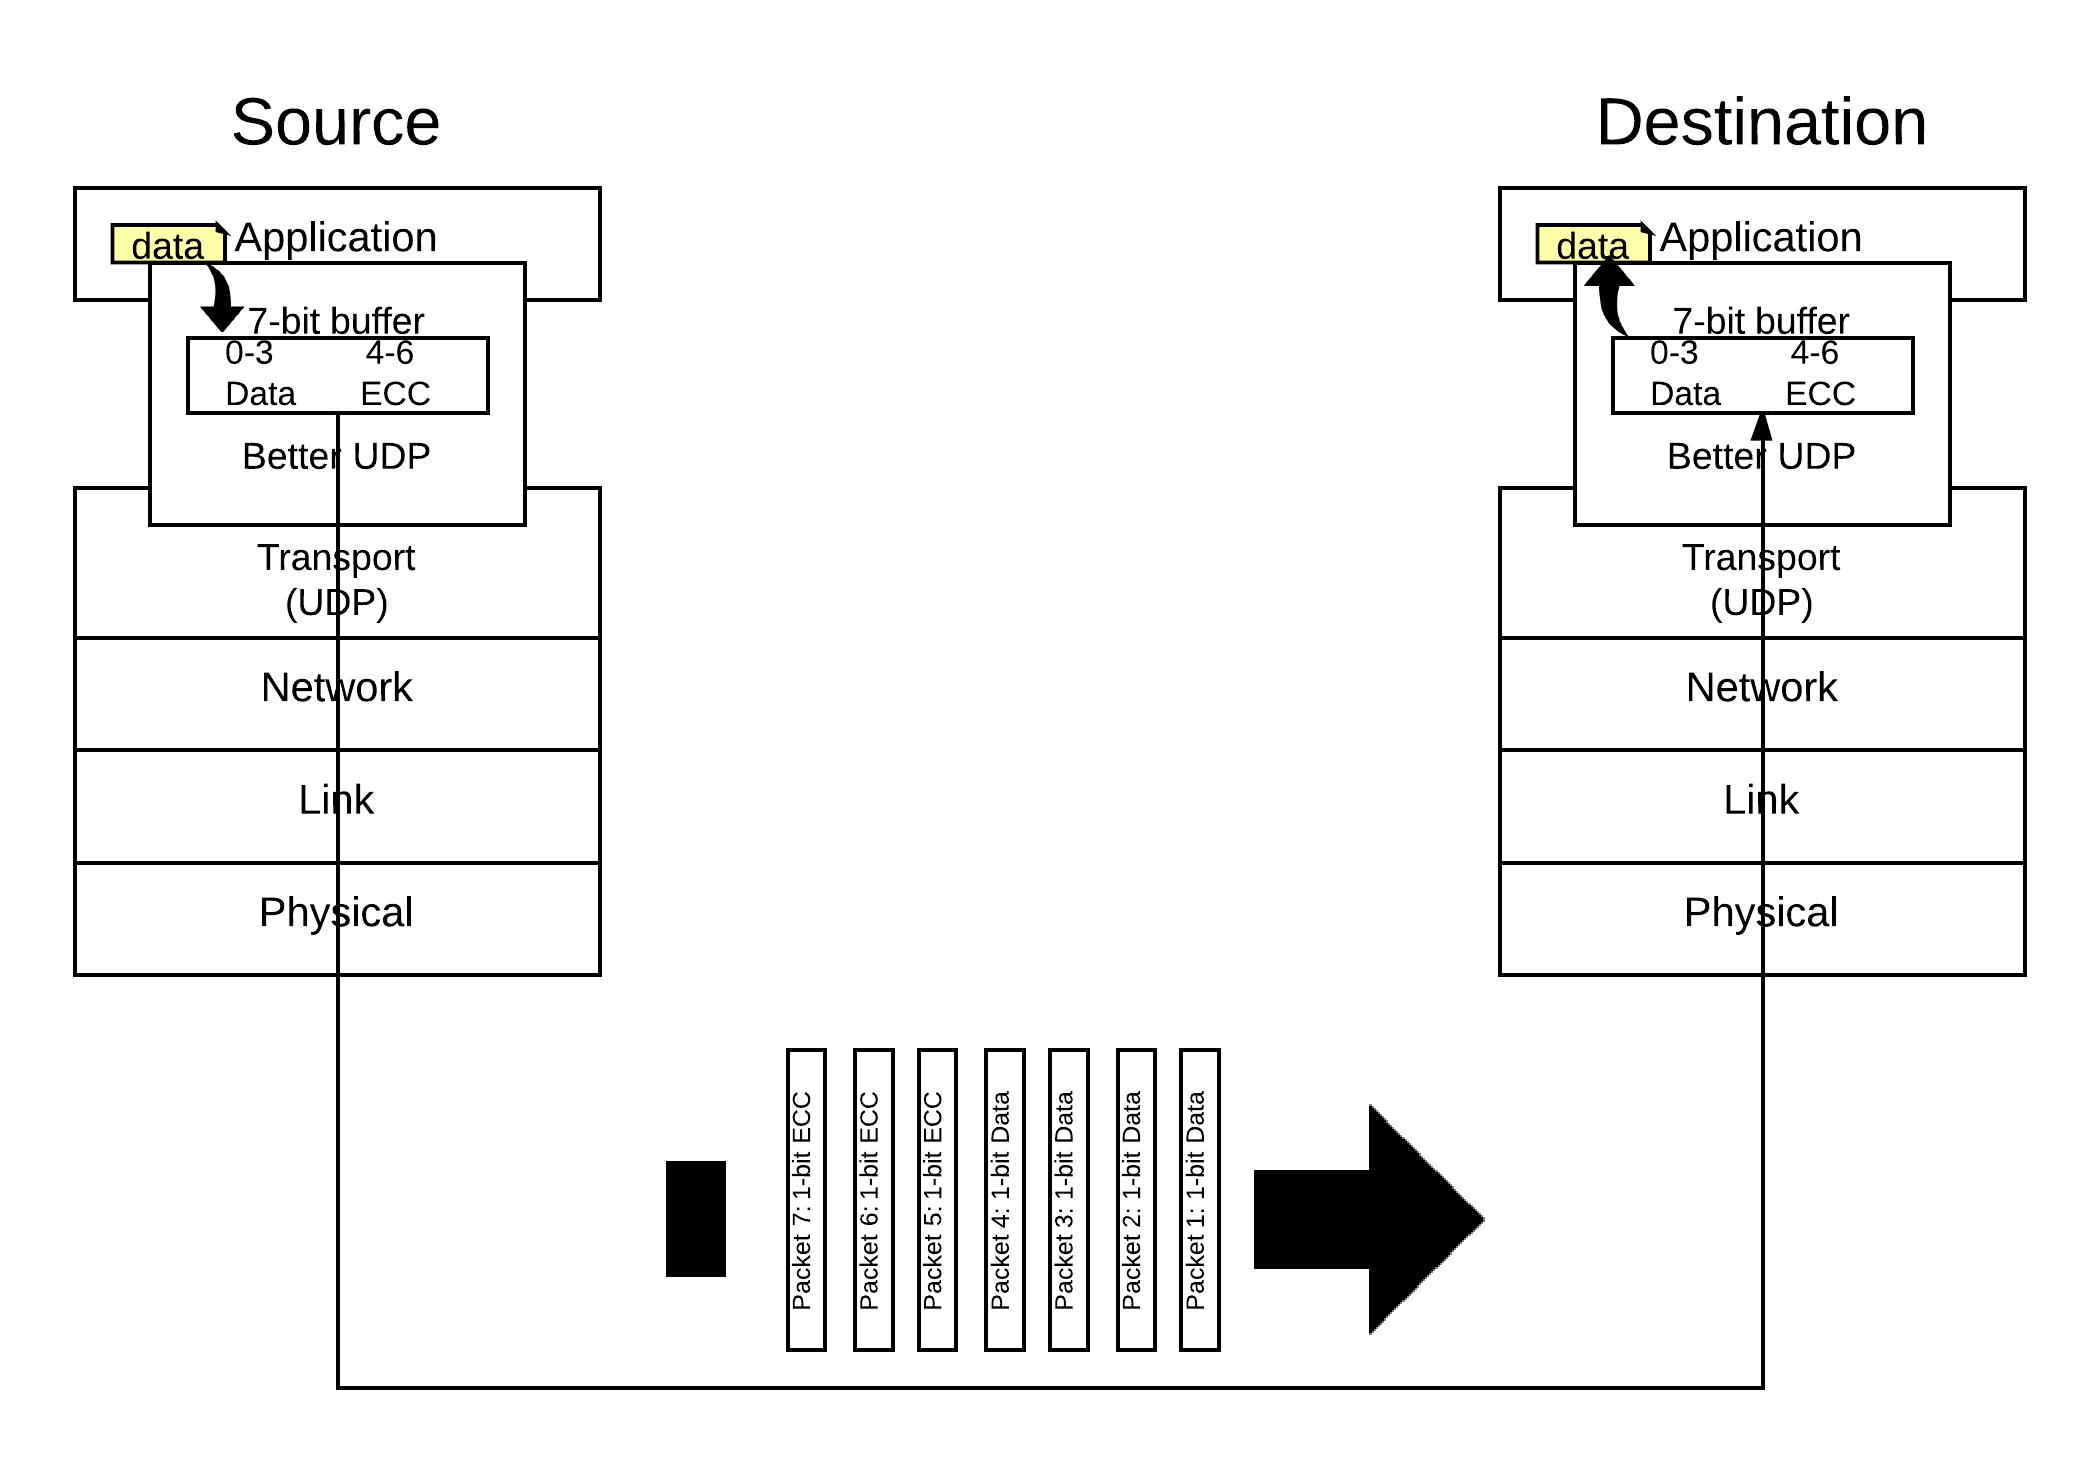
\includegraphics[scale=0.125]{PNGs/System_Schematic-Overview}             %%%%
\caption{A Better UDP Overview Diagram}                                   %%%%
\label{overview_schematic}                                                  %%%%
\end{figure}                                                                %%%%
%%%%                                                                        %%%%
%%%%                                                                        %%%%
%%%%    A BETTER UDP OVERVIEW SCHEMATIC - END                               %%%%
%%%%                                                                        %%%%
%%%%************************************************************************%%%%

The second condition which can prompt message
delivery to the application layer (i.e. condition 2)
above) requires the use of Error-Correcting Codes.
For the purposes of prototyping our design, we
used the single error-correcting Hamming
code introduced above which allowed us to benchmark
our implementation against both standard TCP and
standard UDP.
%In general, a more robust
%and scalable ECC, like Reed-Solomon which is discussed
%in RFC5510 \cite{lacan2009reed}, should be used, as the
%code we used is quite limited and so we had to keep
%our message size unrealistically small, 1-bit.
%For our design the [7,4,3] Hamming code serves as a
%placeholder until Reed-Solomon can be integrated.
%In general, a more robust
%and scalable ECC, like Reed-Solomon which is discussed
%in RFC5510 \cite{lacan2009reed}, should be used, as the
%code we used is quite limited and so we had to keep
%our message size unrealistically small, 1-bit.
%For our design the [7,4,3] Hamming code serves as a
%placeholder until Reed-Solomon can be integrated.
%Nonetheless, the use of the Hamming code will
%allow us to benchmark our design against both
%standard TCP and standard UDP.
Our purposes for using this code over the Reed-Solomon code
suggested in RFC5510\cite{lacan2009reed} were four-fold:

\begin{enumerate}
 \item It is simple to implement and suits our purposes very well.
 \item One of our co-author was very familiar with it
       and its connection to Finite Geometry.
 \item The [7,4,3] Hamming code is a perfect single error-correcting
       code, which happens to be the smallest perfect code,
       and is generated by a finite geometry known
       as the Fano Plane which is the smallest
       projective plane\cite{clanton2005maa}.
 \item Looking long term, we perhaps want to move
       our implementation to the newer so-called
       ``Low-Density Parity-Check Codes'' which
       have been beating some of the more recent ECC
       frontrunners such as turbo codes in competitions\cite{kou2001low}.
       Some of these codes can be generated from Finite
       Geometries, and those that are ``can be decoded in various
       ways, ranging from low to high decoding complexity and from
       reasonably good to very good performance''\cite{kou2001low}.
\end{enumerate}


Encoding the message stream, using four messages
at a time, produces a 3-bit ECC, which is essentially
a concatenation onto the four data bits coming from the
source application layer.  These ECC bits are sent in
three follow-on datagrams to the destination. These
datagrams also contain sequence numbers, which are a
continuation of the sequence numbers assigned to
data/message datagrams.  To use the [7,4,3] Hamming
code, there are two very important matrices required:
the \emph{generator matrix} $G$

$$
G = \left( 
\begin{matrix}
  1 & 0 & 0 & 0 & 1 & 1 & 0 \\
  0 & 1 & 0 & 0 & 1 & 0 & 1 \\
  0 & 0 & 1 & 0 & 0 & 1 & 1 \\
  0 & 0 & 0 & 1 & 1 & 1 & 1
 \end{matrix}
\right)
$$

and the \emph{parity-check matrix} $H$

$$
H = \left( 
\begin{matrix}
  1 & 1 & 0 & 1 & 1 & 0 & 0 \\
  1 & 0 & 1 & 1 & 0 & 1 & 0 \\
  0 & 1 & 1 & 1 & 0 & 0 & 1
 \end{matrix}
\right)
$$


At the source, to encode a message $m$, which for purposes
of the math is represented as a row vector in $\mathbf{F}^4_2$,
multiply it on the right by $G$ to get $mG$, which is
a row vector in $\mathbf{F}^7_2$, where the first four
coordinates are $m$ and the last 3 coordinates are the
parity-check bits, or (as we have been referring to
them) the ``ECC''.  In \cite{lacan2009reed}, these bits
are called repair symbols.

At the destination, to decode the received vector $r\in\mathbf{F}^7_2$,
mutliply it on the right by $H^\text{T}$ to get $rH^\text{T}$, which is
a row vector in $\mathbf{F}^3_2$ known as the syndrome.  Next, syndrome
decoding is performed whereby a \emph{coset leader} $e$ is matched
with the syndrome $rH$. This coset leader represents the error vector
between the received vector $r$ and the closet codeword $c$ to it. To
determine $c$ simply add $r$ and $e$ modulo 2.  That is,

$$
c = r + e\; \mod 2
$$


%%%%************************************************************************%%%%
%%%%                                                                        %%%%
%%%%     One Level - Outer ECC - BEGIN                                      %%%%
%%%%                                                                        %%%%
%%%%                                                                        %%%%
\begin{figure}[t!]                                                          %%%%
\centering                                                                  %%%%
\resizebox{0.4\textwidth}{!}{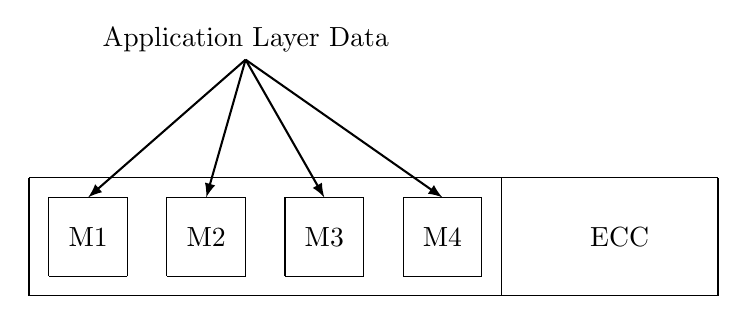
\begin{tikzpicture}
  \node [style=none] (0) at (-2.25, 0.25) {ECC};
  \node [style=none] (1) at (-6.5, 0.75) {};
  \node [style=none] (2) at (-4.5, 0.25) {M4};
  \node [style=none] (3) at (-7, -0.25) {};
  \node [style=none] (4) at (-4, -0.25) {};
  \node [style=none] (5) at (-6.5, -0.25) {};
  \node [style=none] (6) at (-5.5, -0.25) {};
  \node [style=none] (7) at (-8, -0.25) {};
  \node [style=none] (8) at (-9.5, 0.75) {};
  \node [style=none] (9) at (-5, 0.75) {};
  \node [style=none] (10) at (-6, 0.25) {M3};
  \node [style=none] (11) at (-8.5, -0.25) {};
  \node [style=none] (12) at (-4, 0.75) {};
  \node [style=none] (13) at (-3.75, -0.5) {};
  \node [style=none] (14) at (-9, 0.25) {M1};
  \node [style=none] (15) at (-7.5, 0.25) {M2};
  \node [style=none] (16) at (-9.5, -0.25) {};
  \node [style=none] (17) at (-5.5, 0.75) {};
  \node [style=none] (18) at (-5, -0.25) {};
  \node [style=none] (19) at (-3.75, 1) {};
  \node [style=none] (20) at (-9.75, 1) {};
  \node [style=none] (21) at (-9.75, -0.5) {};
  \node [style=none] (22) at (-8, 0.75) {};
  \node [style=none] (23) at (-8.5, 0.75) {};
  \node [style=none] (24) at (-7, 0.75) {};
  \node [style=none] (25) at (-1, 1) {};
  \node [style=none] (26) at (-1, -0.5) {};
  \node [style=none] (27) at (-4.5, 0.75) {};
  \node [style=none] (28) at (-6, 0.75) {};
  \node [style=none] (29) at (-7.5, 0.75) {};
  \node [style=none] (30) at (-9, 0.75) {};
  \node [style=none] (31) at (-7, 2.5) {};
  \node [style=none] (32) at (-7, 2.75) {Application Layer Data};
  \draw [style=simple] (8.center) to (23.center);
  \draw [style=simple] (23.center) to (11.center);
  \draw [style=simple] (11.center) to (16.center);
  \draw [style=simple] (16.center) to (8.center);
  \draw [style=simple] (22.center) to (24.center);
  \draw [style=simple] (24.center) to (3.center);
  \draw [style=simple] (3.center) to (7.center);
  \draw [style=simple] (7.center) to (22.center);
  \draw [style=simple] (1.center) to (17.center);
  \draw [style=simple] (17.center) to (6.center);
  \draw [style=simple] (6.center) to (5.center);
  \draw [style=simple] (5.center) to (1.center);
  \draw [style=simple] (9.center) to (12.center);
  \draw [style=simple] (12.center) to (4.center);
  \draw [style=simple] (4.center) to (18.center);
  \draw [style=simple] (18.center) to (9.center);
  \draw [style=simple] (20.center) to (19.center);
  \draw [style=simple] (19.center) to (13.center);
  \draw [style=simple] (13.center) to (21.center);
  \draw [style=simple] (21.center) to (20.center);
  \draw [style=simple] (13.center) to (26.center);
  \draw [style=simple] (26.center) to (25.center);
  \draw [style=simple] (25.center) to (19.center);
  \draw [style=arrow] (31.center) to (30.center);
  \draw [style=arrow] (31.center) to (28.center);
  \draw [style=arrow] (31.center) to (27.center);
  \draw [style=arrow] (31.center) to (29.center);
\end{tikzpicture}
}
\caption{Simplified ECC Encoding Scheme}                                    %%%%
\label{simplified_ecc_scheme}                                               %%%%
\end{figure}                                                                %%%%
%%%%                                                                        %%%%
%%%%                                                                        %%%%
%%%%     One Level - Outer ECC - END                                        %%%%
%%%%                                                                        %%%%
%%%%************************************************************************%%%%


Figure \ref{simplified_ecc_scheme}
shows a simplified diagram of the ECC encoding scheme we implemented,
where `M' stands for message and the number is the datagram
sequence number.  There are actually two levels of ECCs
that we envisioned using, but due to the limited time we
had to spend on this project we were not able to get the
full implementation finished.  The level we implemented,
which is show in Figure, is the so-called outer or
stream level ECC encoding and requires having the payload
data in buffer which is treated as a vector in $\mathbf{F}^7$
in the mathematics of the encoding process.  The second level
is the so-called inner or message level ECC encoding.  This
inner ECC would allow for checking and correcting datagram
integrity.  That is, if a data were received at the destination
for found to be corrupted, it could be ``fixed''.  This
is something that would be much more possible with a 
Reed-Solomon encoding scheme.  Figure \ref{two_level_scheme}
shows how the two level ECC scheme would look.  Although,
to make a scheme like this work the inner ECC has to have
almost as bits as there are data bits.  The reason for this
is because in the case of a lost datagram the outer ECC will
have to regenerate the missing inner ECC.  Once this inner
ECC is regenerated, it will then be used to regenerate
the missing data payload (from scratch).  The amount
of redunduncy in the ECC will be roughly equal the size of
the data.  Our initial thought on this is that it will
force a fixed-size payload, so that the size of the inner
ECC can be pre-determined, but once this two-level scheme
is prototyped we may find this isn't the case.


%%%%************************************************************************%%%%
%%%%                                                                        %%%%
%%%%    Two-level ECC Encoding Scheme - BEGIN                               %%%%
%%%%                                                                        %%%%
%%%%                                                                        %%%%
\begin{figure}[h!]                                                          %%%%
\centering                                                                  %%%%
\resizebox{0.4\textwidth}{!}{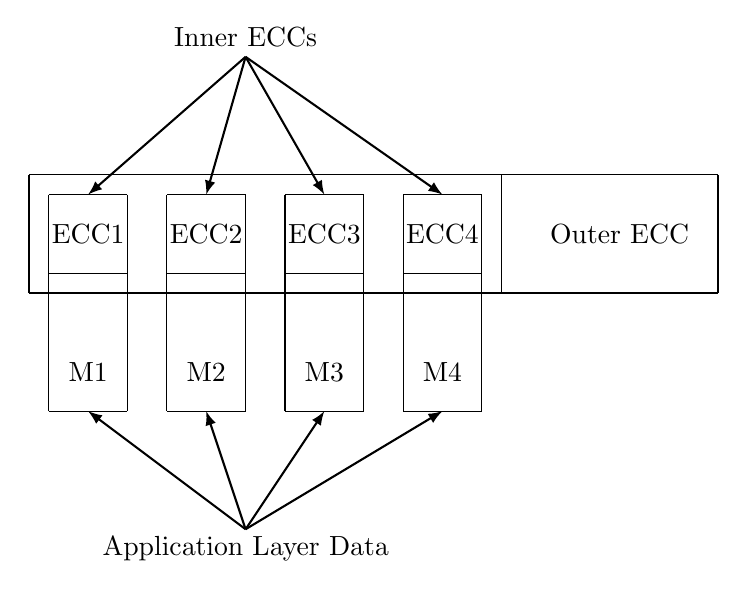
\begin{tikzpicture}
  \node [style=none] (0) at (-2.25, 0.25) {Outer ECC};
  \node [style=none] (1) at (-6.5, 0.75) {};
  \node [style=none] (2) at (-4.5, -1.5) {M4};
  \node [style=none] (3) at (-7, -0.25) {};
  \node [style=none] (4) at (-4, -0.25) {};
  \node [style=none] (5) at (-6.5, -0.25) {};
  \node [style=none] (6) at (-5.5, -0.25) {};
  \node [style=none] (7) at (-8, -0.25) {};
  \node [style=none] (8) at (-9.5, 0.75) {};
  \node [style=none] (9) at (-5, 0.75) {};
  \node [style=none] (10) at (-6, -1.5) {M3};
  \node [style=none] (11) at (-8.5, -0.25) {};
  \node [style=none] (12) at (-4, 0.75) {};
  \node [style=none] (13) at (-3.75, -0.5) {};
  \node [style=none] (14) at (-9, -1.5) {M1};
  \node [style=none] (15) at (-7.5, -1.5) {M2};
  \node [style=none] (16) at (-9.5, -0.25) {};
  \node [style=none] (17) at (-5.5, 0.75) {};
  \node [style=none] (18) at (-5, -0.25) {};
  \node [style=none] (19) at (-3.75, 1) {};
  \node [style=none] (20) at (-9.75, 1) {};
  \node [style=none] (21) at (-9.75, -0.5) {};
  \node [style=none] (22) at (-8, 0.75) {};
  \node [style=none] (23) at (-8.5, 0.75) {};
  \node [style=none] (24) at (-7, 0.75) {};
  \node [style=none] (25) at (-9.5, -2) {};
  \node [style=none] (26) at (-8.5, -2) {};
  \node [style=none] (27) at (-8, -2) {};
  \node [style=none] (28) at (-7, -2) {};
  \node [style=none] (29) at (-6.5, -2) {};
  \node [style=none] (30) at (-5.5, -2) {};
  \node [style=none] (31) at (-5, -2) {};
  \node [style=none] (32) at (-4, -2) {};
  \node [style=none] (33) at (-9, 0.25) {ECC1};
  \node [style=none] (34) at (-7.5, 0.25) {ECC2};
  \node [style=none] (35) at (-6, 0.25) {ECC3};
  \node [style=none] (36) at (-4.5, 0.25) {ECC4};
  \node [style=none] (37) at (-1, 1) {};
  \node [style=none] (38) at (-1, -0.5) {};
  \node [style=none] (39) at (-4.5, 0.75) {};
  \node [style=none] (40) at (-7, 2.5) {};
  \node [style=none] (41) at (-6, 0.75) {};
  \node [style=none] (42) at (-7.5, 0.75) {};
  \node [style=none] (43) at (-9, 0.75) {};
  \node [style=none] (44) at (-7, 2.75) {Inner ECCs};
  \node [style=none] (45) at (-7, -3.5) {};
  \node [style=none] (46) at (-9, -2) {};
  \node [style=none] (47) at (-7.5, -2) {};
  \node [style=none] (48) at (-6, -2) {};
  \node [style=none] (49) at (-4.5, -2) {};
  \node [style=none] (50) at (-7, -3.75) {Application Layer Data};
  \draw [style=simple] (8.center) to (23.center);
  \draw [style=simple] (23.center) to (11.center);
  \draw [style=simple] (11.center) to (16.center);
  \draw [style=simple] (16.center) to (8.center);
  \draw [style=simple] (22.center) to (24.center);
  \draw [style=simple] (24.center) to (3.center);
  \draw [style=simple] (3.center) to (7.center);
  \draw [style=simple] (7.center) to (22.center);
  \draw [style=simple] (1.center) to (17.center);
  \draw [style=simple] (17.center) to (6.center);
  \draw [style=simple] (6.center) to (5.center);
  \draw [style=simple] (5.center) to (1.center);
  \draw [style=simple] (9.center) to (12.center);
  \draw [style=simple] (12.center) to (4.center);
  \draw [style=simple] (4.center) to (18.center);
  \draw [style=simple] (18.center) to (9.center);
  \draw [style=simple] (20.center) to (19.center);
  \draw [style=simple] (19.center) to (13.center);
  \draw [style=simple] (13.center) to (21.center);
  \draw [style=simple] (21.center) to (20.center);
  \draw [style=simple] (16.center) to (25.center);
  \draw [style=simple] (25.center) to (26.center);
  \draw [style=simple] (26.center) to (11.center);
  \draw [style=simple] (7.center) to (27.center);
  \draw [style=simple] (27.center) to (28.center);
  \draw [style=simple] (28.center) to (3.center);
  \draw [style=simple] (5.center) to (29.center);
  \draw [style=simple] (29.center) to (30.center);
  \draw [style=simple] (30.center) to (6.center);
  \draw [style=simple] (31.center) to (18.center);
  \draw [style=simple] (31.center) to (32.center);
  \draw [style=simple] (32.center) to (4.center);
  \draw [style=simple] (13.center) to (38.center);
  \draw [style=simple] (38.center) to (37.center);
  \draw [style=simple] (37.center) to (19.center);
  \draw [style=arrow] (40.center) to (39.center);
  \draw [style=arrow] (40.center) to (41.center);
  \draw [style=arrow] (40.center) to (42.center);
  \draw [style=arrow] (40.center) to (43.center);
  \draw [style=arrow] (45.center) to (46.center);
  \draw [style=arrow] (45.center) to (47.center);
  \draw [style=arrow] (45.center) to (48.center);
  \draw [style=arrow] (45.center) to (49.center);
\end{tikzpicture}
}
\caption{Two-level ECC Encoding Scheme}                                     %%%%
\label{two_level_scheme}                                                    %%%%
\end{figure}                                                                %%%%
%%%%                                                                        %%%%
%%%%                                                                        %%%%
%%%%    Two-level ECC Encoding Scheme - END                                 %%%%
%%%%                                                                        %%%%
%%%%************************************************************************%%%%


Our BUDP datagram will be encapsulated in an ordinary
UDP datagram.  More specifically, BUDP will contain a
header including a field for the sequence number and
a field for an ECC flag, indicating whether the
payload holds an ECC or data.  This BUDP datagram
(BUDP header + BUDP payload), will form the payload
of a regular UDP datagram.  See Figure \ref{budp_encap}
below.

\begin{figure}[h!]
\centering
\resizebox{0.45\textwidth}{!}{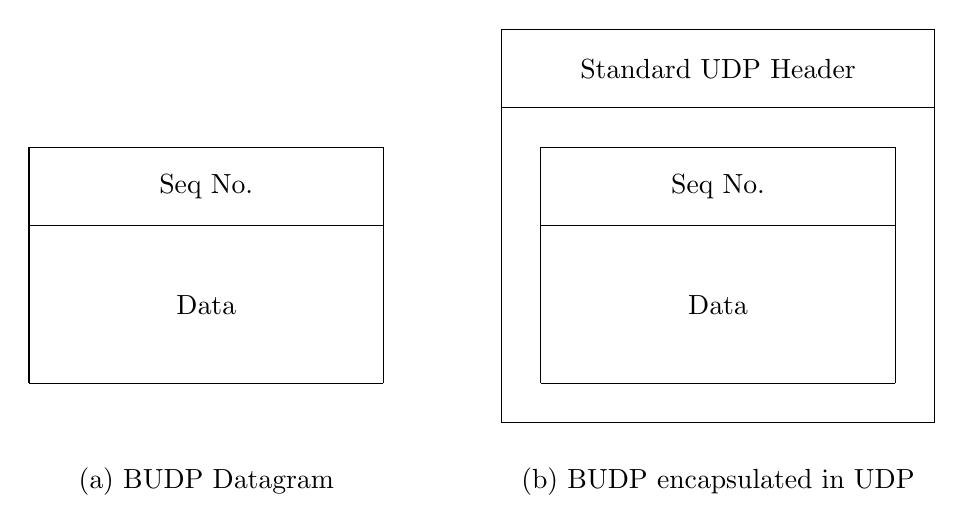
\begin{tikzpicture}
  \node [style=none] (0) at (-6.5, 2.25) {};
  \node [style=none] (1) at (-2, 2.25) {};
  \node [style=none] (2) at (-6.5, 1.25) {};
  \node [style=none] (3) at (-2, 1.25) {};
  \node [style=none] (4) at (-6.5, -0.75) {};
  \node [style=none] (5) at (-2, -0.75) {};
  \node [style=none] (6) at (-4.25, 1.75) {Seq No.};
  \node [style=none] (7) at (-4.25, 0.25) {Data};
  \node [style=none] (8) at (4.5, 1.25) {};
  \node [style=none] (9) at (4.5, 2.25) {};
  \node [style=none] (10) at (0, -0.75) {};
  \node [style=none] (11) at (2.25, 0.25) {Data};
  \node [style=none] (12) at (0, 2.25) {};
  \node [style=none] (13) at (0, 1.25) {};
  \node [style=none] (14) at (4.5, -0.75) {};
  \node [style=none] (15) at (2.25, 1.75) {Seq No.};
  \node [style=none] (16) at (-0.5, -1.25) {};
  \node [style=none] (17) at (5, -1.25) {};
  \node [style=none] (18) at (5, 2.75) {};
  \node [style=none] (19) at (2.25, 3.25) {Standard UDP Header};
  \node [style=none] (20) at (-0.5, 2.75) {};
  \node [style=none] (21) at (5, 3.75) {};
  \node [style=none] (22) at (-0.5, 3.75) {};
  \node [style=none] (23) at (-4.25, -2) {(a) BUDP Datagram};
  \node [style=none] (24) at (2.25, -2) {(b) BUDP encapsulated in UDP};
  \draw [style=simple] (1.center) to (3.center);
  \draw [style=simple] (2.center) to (0.center);
  \draw [style=simple] (2.center) to (4.center);
  \draw [style=simple] (4.center) to (5.center);
  \draw [style=simple] (5.center) to (3.center);
  \draw [style=simple] (9.center) to (8.center);
  \draw [style=simple] (13.center) to (12.center);
  \draw [style=simple] (13.center) to (10.center);
  \draw [style=simple] (10.center) to (14.center);
  \draw [style=simple] (14.center) to (8.center);
  \draw [style=simple] (16.center) to (17.center);
  \draw [style=simple] (17.center) to (18.center);
  \draw [style=simple] (18.center) to (21.center);
  \draw [style=simple] (21.center) to (22.center);
  \draw [style=simple] (22.center) to (20.center);
  \draw [style=simple] (20.center) to (16.center);
  \draw [style=simple] (20.center) to (18.center);
  \draw (0.center) to (1.center);
  \draw (2.center) to (3.center);
  \draw (13.center) to (8.center);
  \draw (12.center) to (9.center);
\end{tikzpicture}
}
\caption{BUDP Encapsulation}
\label{budp_encap}
\end{figure}


\section{Results}
We expected our our implementation to perform at
about half the throughput of stock UDP, due to the
fact that there nearly as many redundancy bits
as there are data bits.  What we were curious to
see is how well it fared compared to standard TCP.

To run these benchmarks, we forced datagrams to be
drop via....

Need to talk about information rates, how to improve
these, how newest codes will solve issues


%%%%************************************************************************%%%%
%%%%                                                                        %%%%
%%%%     - BEGIN                             %%%%
%%%%                                                                        %%%%
%%%%                                                                        %%%%
%\begin{figure}[h!]                                                          %%%%
%\centering                                                                  %%%%
%  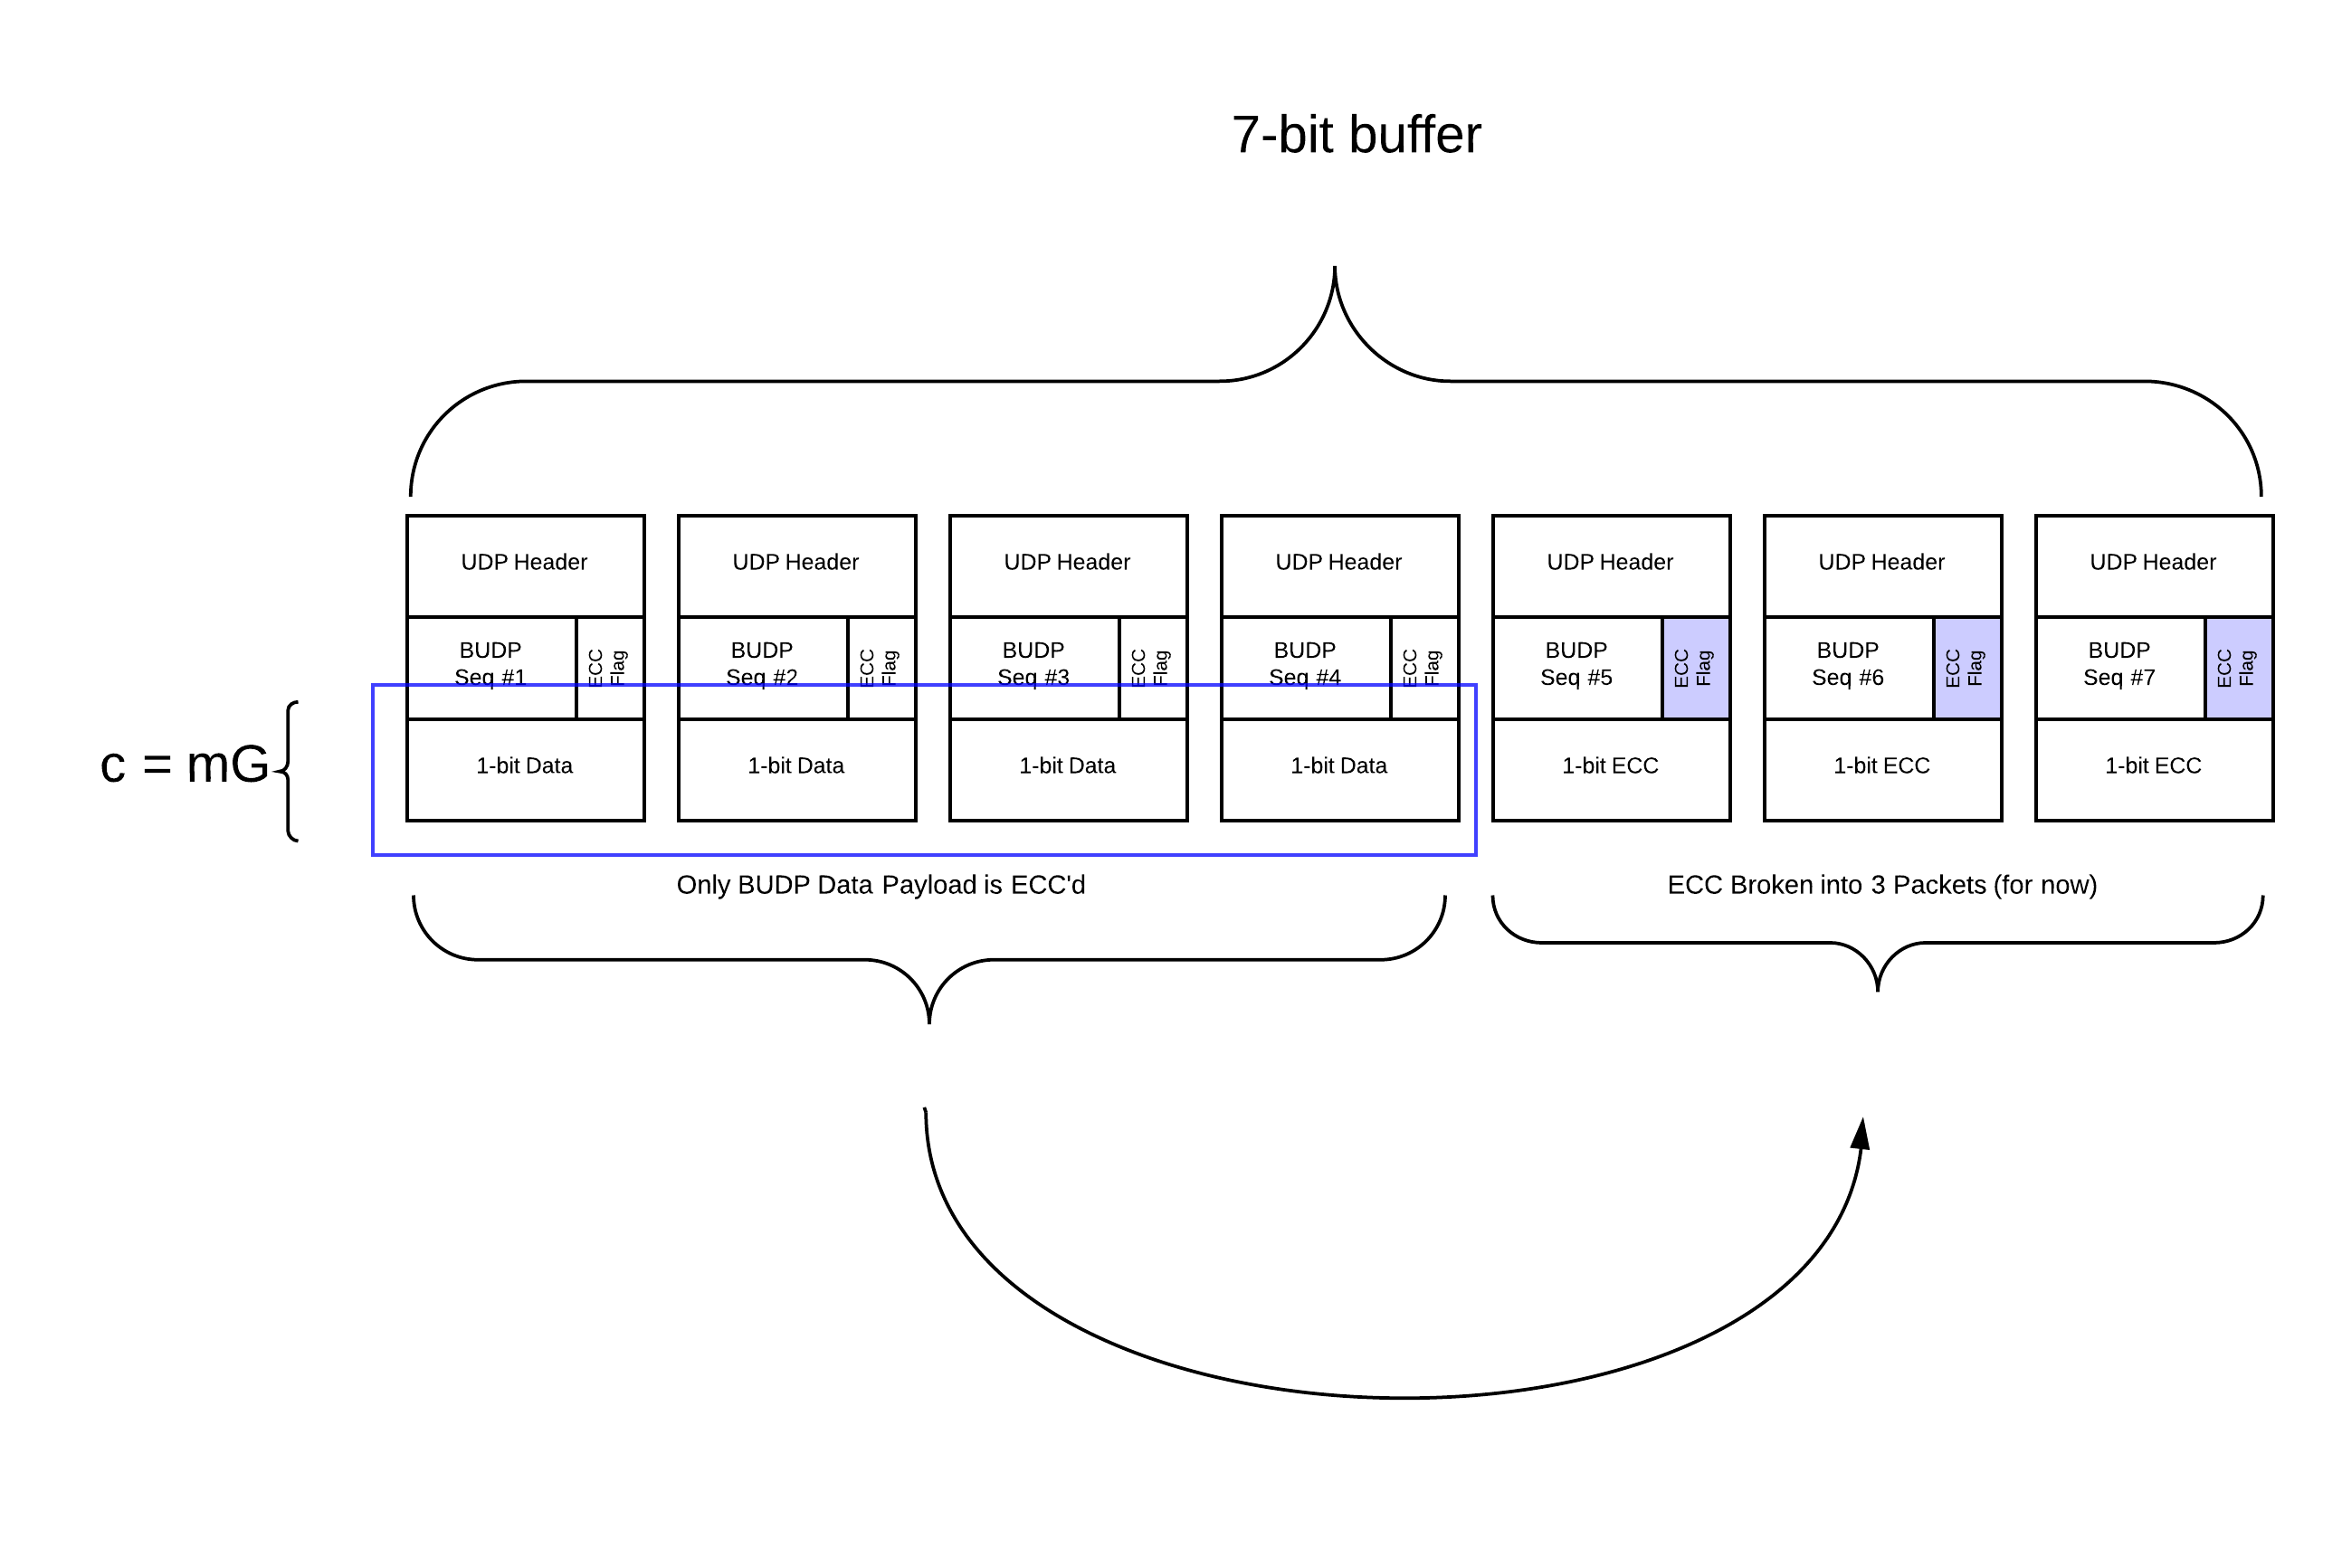
\includegraphics[scale=0.075]{PNGs/Buffer_and_Stream_Level_ECC}           %%%%
%\caption{Prototype ECC encoding scheme}                                     %%%%
%\label{proto_ecc_scheme}                                                    %%%%
%\end{figure}                                                                %%%%
%%%%                                                                        %%%%
%%%%                                                                        %%%%
%%%%     - END                               %%%%
%%%%                                                                        %%%%
%%%%************************************************************************%%%%



%Subsubsection text here.


% An example of a floating figure using the graphicx package.
% Note that \label must occur AFTER (or within) \caption.
% For figures, \caption should occur after the \includegraphics.
% Note that IEEEtran v1.7 and later has special internal code that
% is designed to preserve the operation of \label within \caption
% even when the captionsoff option is in effect. However, because
% of issues like this, it may be the safest practice to put all your
% \label just after \caption rather than within \caption{}.
%
% Reminder: the "draftcls" or "draftclsnofoot", not "draft", class
% option should be used if it is desired that the figures are to be
% displayed while in draft mode.
%
%\begin{figure}[!t]
%\centering
%\includegraphics[width=2.5in]{myfigure}
% where an .eps filename suffix will be assumed under latex, 
% and a .pdf suffix will be assumed for pdflatex; or what has been declared
% via \DeclareGraphicsExtensions.
%\caption{Simulation Results}
%\label{fig_sim}
%\end{figure}

% Note that IEEE typically puts floats only at the top, even when this
% results in a large percentage of a column being occupied by floats.


% An example of a double column floating figure using two subfigures.
% (The subfig.sty package must be loaded for this to work.)
% The subfigure \label commands are set within each subfloat command, the
% \label for the overall figure must come after \caption.
% \hfil must be used as a separator to get equal spacing.
% The subfigure.sty package works much the same way, except \subfigure is
% used instead of \subfloat.
%
%\begin{figure*}[!t]
%\centerline{\subfloat[Case I]\includegraphics[width=2.5in]{subfigcase1}%
%\label{fig_first_case}}
%\hfil
%\subfloat[Case II]{\includegraphics[width=2.5in]{subfigcase2}%
%\label{fig_second_case}}}
%\caption{Simulation results}
%\label{fig_sim}
%\end{figure*}
%
% Note that often IEEE papers with subfigures do not employ subfigure
% captions (using the optional argument to \subfloat), but instead will
% reference/describe all of them (a), (b), etc., within the main caption.


% An example of a floating table. Note that, for IEEE style tables, the 
% \caption command should come BEFORE the table. Table text will default to
% \footnotesize as IEEE normally uses this smaller font for tables.
% The \label must come after \caption as always.
%
%\begin{table}[!t]
%% increase table row spacing, adjust to taste
%\renewcommand{\arraystretch}{1.3}
% if using array.sty, it might be a good idea to tweak the value of
% \extrarowheight as needed to properly center the text within the cells
%\caption{An Example of a Table}
%\label{table_example}
%\centering
%% Some packages, such as MDW tools, offer better commands for making tables
%% than the plain LaTeX2e tabular which is used here.
%\begin{tabular}{|c||c|}
%\hline
%One & Two\\
%\hline
%Three & Four\\
%\hline
%\end{tabular}
%\end{table}


% Note that IEEE does not put floats in the very first column - or typically
% anywhere on the first page for that matter. Also, in-text middle ("here")
% positioning is not used. Most IEEE journals/conferences use top floats
% exclusively. Note that, LaTeX2e, unlike IEEE journals/conferences, places
% footnotes above bottom floats. This can be corrected via the \fnbelowfloat
% command of the stfloats package.



\section{Conclusion}
We have presented a design for a better UDP implementation
where datagrams arrive in-order to the application layer
at the destination and when a datagram is lost it can be
reconstructed, provided 75\% of the datagrams in its ECC
grouping and the ECC arrive intact.  If these latter two
conditions are not met, then BUDP simply hands over what
it does have to the application layer after a countdown
clock expires.

Our results indicate that....


In the future, we would like to integrate a more robust
Error-Correcting Code such as Reed-Solomon as documented
in RFC5510.  Futhermore, we would like to implement the
two-level ECC encoding scheme to build in more redundancy.

Our view is in order to deal with the unreliability inherent
in the Internet Protocol, a designer has to either build
in redunduncy to help clean the communication channel or
(s)he has to build in a retransmission infastructure, as
is the case with TCP.  We prefer the error-correcting redundancy....
or we did the redunduncy since it isn't available otherwise, etc.
etc.

Need to talk about information rates, how to improve
these, how newest codes will solve issues



% conference papers do not normally have an appendix


% use section* for acknowledgement
\section*{Acknowledgment}
The Error-Correct Codes subsection of the Introduction
was taken, in part, from a presentation one of the co-authors
presented at a Mathematical Association of America
Texas Section conference in April 2005 \cite{clanton2005maa}
focusing on its connection to Finite Geometries.
It was included here to help demystify some of the math
related to the [7,4,3] Hamming code used in our prototype.
All other sections and subsections are original.  This is the
first time any of these authors have used Error-Correcting
Codes to improve a transport protocol.




% trigger a \newpage just before the given reference
% number - used to balance the columns on the last page
% adjust value as needed - may need to be readjusted if
% the document is modified later
%\IEEEtriggeratref{8}
% The "triggered" command can be changed if desired:
%\IEEEtriggercmd{\enlargethispage{-5in}}

% references section

% can use a bibliography generated by BibTeX as a .bbl file
% BibTeX documentation can be easily obtained at:
% http://www.ctan.org/tex-archive/biblio/bibtex/contrib/doc/
% The IEEEtran BibTeX style support page is at:
% http://www.michaelshell.org/tex/ieeetran/bibtex/
%\bibliographystyle{IEEEtran}
% argument is your BibTeX string definitions and bibliography database(s)
%\bibliography{IEEEabrv,../bib/paper}
%
% <OR> manually copy in the resultant .bbl file
% set second argument of \begin to the number of references
% (used to reserve space for the reference number labels box)
%\begin{thebibliography}{1}

%\bibitem{IEEEhowto:kopka}
%H.~Kopka and P.~W. Daly, \emph{A Guide to \LaTeX}, 3rd~ed.\hskip 1em plus
%  0.5em minus 0.4em\relax Harlow, England: Addison-Wesley, 1999.

%E.~F. Assmus and J.~D. Key, \emph{DESIGNS AND THEIR CODES}, 3rd~ed.\hskip 1em plus
%  0.5em minus 0.4em\relax Harlow, England: Addison-Wesley, 1999.

%\end{thebibliography}


%\bibliographystyle{plain}
%\bibliography{a_better_udp}

\bibliographystyle{IEEEtran}
\bibliography{IEEEabrv,a_better_udp}


% that's all folks
\end{document}


